\documentclass[style=sailor,size=12pt]{powerdot}
\usepackage{epic,array,ecltree,url,calrsfs}
\usepackage[nointegrals]{wasysym}
\usepackage{listings}
\usepackage{epsfig}
\usepackage{amsmath}
\usepackage{amsfonts}
\usepackage{amssymb}
\usepackage{amsxtra}
\usepackage{amsthm}
\usepackage{mlextra} % Must be below ams packages
\usepackage{mathrsfs}
\usepackage{color}
\usepackage{array}
\usepackage{graphicx}
\graphicspath{ {../art/} }
\usepackage{bm}
\usepackage{tikz}
\usepackage{multicol}
\usepackage{enumitem}

\newcommand{\treenode}{%
  \begingroup\normalfont
  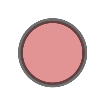
\includegraphics[height=\fontcharht\font`\c]{node.eps}%
  \endgroup
}

\newcommand{\tripletreenode}{%
  \begingroup\normalfont
  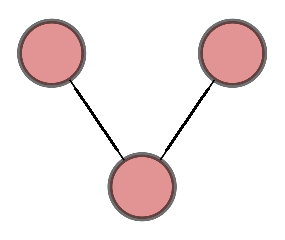
\includegraphics[height=\fontcharht\font`\B]{3nodetree.eps}%
  \endgroup
}

\pdsetup{method=normal}

\title{Systems and Proof: Part I}
\author{Foundations of Computer Science}
\date{\today}

\begin{document}
\maketitle
\begin{slide}[toc=,bm=]{Overview}
This slide set covers the following topics:

\vspace{5mm}
\tableofcontents[content=sections]
\end{slide}

\section[slide=true]{Expressing Recursive Definitions with Post Systems} 
%\documentclass[style=sailor,size=12pt]{powerdot}
%\usepackage{epic,array,ecltree,url}
%\usepackage[nointegrals]{wasysym}
%\usepackage{mathtools}
%\usepackage{graphicx}
%\graphicspath{ {../art/} }
%\usepackage[labelformat=empty]{caption}
%
%\newcommand{\id}[1]{\mbox{\it #1\/}}
%\newcommand{\rid}[1]{\mbox{\rm #1}}
%\newcommand{\sid}[1]{\mbox{\sf #1}}
%\newcommand{\bid}[1]{\mbox{\bf #1}}
%\newcommand{\tinysz}[1]{\mbox{\tiny $#1$}}
%
%\newcommand{\lra}{\longrightarrow}
%\newcommand{\ra}{\rightarrow}
%\newcommand{\surj}{\twoheadrightarrow}
%\newcommand{\graph}{\mathrm{graph}}
%\newcommand{\bb}[1]{\mathbb{#1}}
%\newcommand{\Ell}{\mathscr{L}}
%\newcommand{\Z}{\bb{Z}}
%\newcommand{\Q}{\bb{Q}}
%\newcommand{\R}{\bb{R}}
%\newcommand{\C}{\bb{C}}
%\newcommand{\N}{\bb{N}}
%\newcommand{\M}{\mathbf{M}}
%\newcommand{\m}{\mathbf{m}}
%\newcommand{\MM}{\mathscr{M}}
%\newcommand{\HH}{\mathscr{H}}
%\newcommand{\Om}{\Omega}
%\newcommand{\Ho}{\in\HH(\Om)}
%\newcommand{\bd}{\partial}
%\newcommand{\del}{\partial}
%\newcommand{\bardel}{\overline\partial}
%\newcommand{\textdf}[1]{\textbf{\textsf{#1}}\index{#1}}
%\newcommand{\img}{\mathrm{img}}
%\newcommand{\ip}[2]{\left\langle{#1},{#2}\right\rangle}
%\newcommand{\inter}[1]{\mathrm{int}{#1}}
%\newcommand{\exter}[1]{\mathrm{ext}{#1}}
%\newcommand{\cl}[1]{\mathrm{cl}{#1}}
%\newcommand{\ds}{\displaystyle}
%\newcommand{\vol}{\mathrm{vol}}
%\newcommand{\cnt}{\mathrm{ct}}
%\newcommand{\osc}{\mathrm{osc}}
%\newcommand{\LL}{\mathbf{L}}
%\newcommand{\UU}{\mathbf{U}}
%\newcommand{\support}{\mathrm{support}}
%\newcommand{\AND}{\;\wedge\;}
%\newcommand{\OR}{\;\vee\;}
%\newcommand{\Oset}{\varnothing}
%\newcommand{\st}{\ni}
%\newcommand{\wh}{\widehat}
%\newcommand{\mli}[1]{\mathit{#1}}
%\newcommand{\ndiv}{\hspace{-3pt}\not|\hspace{2pt}}

%\newcommand{\node}{%
%  \begingroup\normalfont
%  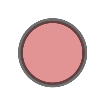
\includegraphics[height=\fontcharht\font`\c]{node.eps}%
%  \endgroup
%}
%
%\newcommand{\threenode}{%
%  \begingroup\normalfont
%  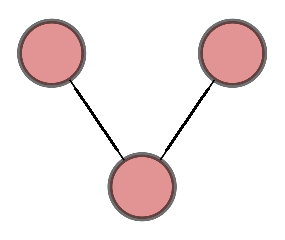
\includegraphics[height=\fontcharht\font`\B]{3nodetree.eps}%
%  \endgroup
%}

\begin{wideslide}[bm=,toc=]{Models of computation}
\begin{itemize}
\item Different computational models have been developed independently:
%\item Machine independent: recursive function theory.
%\item Machine dependent:
\begin{enumerate}
\item Turing machines, Alan Turing (covered in CS3101)
\item Lambda calculus, Alonzo Church
\item Post systems, Emil Post
\item and others.
\end{enumerate}
\item Post systems are of interest to us.
\item They can be used to define something (data structure, program).
\item Definitions may be recursive 

\hspace{2em}$A \equiv \ldots A\ldots$

or mutually recursive

\hspace{2em}$A \equiv \ldots B\ldots$

\hspace{2em}$B \equiv \ldots A\ldots$

\item Post systems admit formal proofs---is a definition correct?
\end{itemize}
\end{wideslide}

\begin{wideslide}[bm=,toc=]{Recursive definitions}
\begin{itemize}
\item A recursive definition can be represented in a {\em Post system\/}.
\item Named after mathematician Emil Leon Post.
\item A Post system comprises a finite set of {\em variables\/}, {\em signs\/} and {\em productions\/} 
(inference rules).
\item An inference rule has the form
\begin{displaymath}
\begin{array}{c}
t_1\;t_2\;\cdots\;t_n\\
\hline
t
\end{array}
\end{displaymath}
where $t,t_1,\ldots ,t_n$ ($n\geq 0$) are terms (strings of signs and variables).
\item $t_1,\ldots , t_n$ are the {\em antecedents\/} and $t$ the {\em consequent\/} or conclusion.
\item When $n=0$, an inference rule is called an {\em axiom\/}.
\end{itemize}
\end{wideslide}

\begin{wideslide}[bm=,toc=]{Recursive definitions}
\begin{itemize}
\item A Post system of two productions:
\vspace{-1em}
\begin{tabbing}
{\bf R}XX \=  \kill
{\bf B} \>
        \(\begin{array}[t]{l}
        3\in S
        \end{array}\) \\[2ex]
{\bf R} \>
        \(\begin{array}[t]{l}
        x \in S \;\;\;y \in S \\
        \hline
        x + y \in S
        \end{array}\)
\end{tabbing}
\item The set of signs is $\{3,\in,+\}$ and variables $\{x,y\}$.
\item Claim: system defines the set of all positive multiples of 3.
\item Must prove $n\in S$ iff $n$ is a positive multiple of 3.
\item ``$n\in S$ only if $n$ is a positive multiple of 3'' (system {\em soundness\/}).
\item ``$n\in S$ if $n$ is a positive multiple of 3'' (system {\em completeness\/}).
\end{itemize}
\end{wideslide}
\begin{wideslide}[bm=,toc=]{Example derivation showing $9 \in S$}
\begin{center}
\begin{tabular}{lllll}
  \onslide{2-}{$\bid{B}$  & $\id{3}\in \id{S}$}           & \onslide{3-}{$\id{3}\in \id{S}$ & $\bid{B}$}
  \onslide{4-}{\\ \cline{2-3}}
  \onslide{5-}{$\bid{R}$  & $\id{3} + \id{3} \in \id{S}$} &                    & \onslide{6-}{$\id{3}\in \id{S}$ & $\bid{B}$} 
  \onslide{7-}{\\ \cline{2-4}} 
  \onslide{8-}{$\bid{R}$  & $\id{3} + \id{3} + \id{3} \in \id{S}$ &           & &  \\} 
\end{tabular}
\end{center}

\end{wideslide}
\begin{wideslide}[bm=,toc=]{Recursive Definitions}
\begin{itemize}
\item A Post system with multiple axioms.
\begin{tabbing}
{\bf R1}XX \=  \kill
{\bf B1} \>
        \(\begin{array}[t]{l}
        4\in P
        \end{array}\) \\[2ex]
{\bf B2} \>
        \(\begin{array}[t]{l}
        5\in P
        \end{array}\) \\[2ex]
        
{\bf R} \>
        \(\begin{array}[t]{l}
        x \in P \;\;\;y \in P \\
        \hline
        x + y \in P
        \end{array}\)
\end{tabbing}
\item Claim: every amount of postage at least $12$ can be formed using only $4$
and $5$-cent stamps (Rosen pg. 337).
\item Must show every positive integer at least $12$ belongs to $P$. 
equal to 12.
\item This is a completeness result of the system.
\end{itemize}
\end{wideslide}

\begin{wideslide}[bm=,toc=]{Recursive Definitions}
\begin{itemize}
\item  Another Post system with multiple axioms.
\begin{tabbing}
{\bf R1}XX \=  \kill
{\bf B1} \>
        \(\begin{array}[t]{l}
        \epsilon \in \id{Pal}
        \end{array}\) \\[2ex]
{\bf B2} \>
        \(\begin{array}[t]{l}
        a\in \id{Pal}
        \end{array}\) \\[2ex]

 {\bf B3} \>
        \(\begin{array}[t]{l}
        b\in \id{Pal}
        \end{array}\) \\[2ex]
        
{\bf R} \>
        \(\begin{array}[t]{l}
        x \in \id{Pal} \;\;\;y \in \id{Pal} \\
        \hline
        x(yx) \in \id{Pal}
        \end{array}\)
\end{tabbing}
\item Claim:  $\id{Pal}$ defines exactly the set of palindromes over $\{a,b\}^*$.
\end{itemize}
\end{wideslide}

\begin{wideslide}[bm=,toc=]{Recursive Definitions}
\begin{itemize}
\item  A Post system with multiple recursive rules.
\begin{tabbing}
{\bf R1}XX \=  \kill
{\bf B} \>
        \(\begin{array}[t]{l}
        \epsilon \in \id{X}
        \end{array}\) \\[2ex]

{\bf R1} \>
        \(\begin{array}[t]{l}
        x\in \id{X} \\
        \hline
        1x0 \in \id{X}
        \end{array}\) \\[2ex]

{\bf R2} \>
        \(\begin{array}[t]{l}
        x\in \id{X} \\
        \hline
        0x1 \in \id{X}
        \end{array}\) \\[2ex]
       
{\bf R3} \>
        \(\begin{array}[t]{l}
        x \in \id{X} \;\;\;y \in \id{X} \\
        \hline
        xy \in \id{X}
        \end{array}\)
\end{tabbing}
\item Claim: for all $y \in \{0,1\}^*$, $y \in \id{X}$ iff $y$ has an equal
number of $0$s and $1$s.
\item Rule $\bid{R3}$ is needed to show $1001 \in \id{X}$, for instance.
\end{itemize}
\end{wideslide}

\begin{wideslide}[bm=,toc=]{Recursive definitions}
\begin{itemize}
\item A Post system recursively defining the set {\em P\/} of all well-formed formulae in propositional logic:
\begin{displaymath}
\begin{array}{lll}
        \begin{array}[t]{l}
        \bid{T}\in P
        \end{array}
&
        \begin{array}[t]{l}
        \bid{F}\in P
        \end{array}
&
	\begin{array}[t]{l}
        x \in P \\
        \hline
        \neg x \in P
        \end{array} \\[6ex]

	\begin{array}[t]{l}
	x \in P \;\;y \in P \\
	\hline
	x \wedge y \in P
	\end{array}
&
	\begin{array}[t]{l}
	x \in P \;\;y \in P \\
	\hline
	x \vee y \in P
	\end{array}
&
	\begin{array}[t]{l}
	x \in P \;\;y \in P \\
	\hline
	x \Rightarrow y \in P
	\end{array} \\[6ex]

	\begin{array}[t]{l}
        x \in \id{Var} \\
        \hline
        x \in P
        \end{array}
\end{array}
\end{displaymath}
%\item Consequents have larger terms than antecedents except in last rule.
\end{itemize}
\end{wideslide}

\begin{wideslide}[bm=,toc=]{Rooted trees in Rosen 7th Ed.}
  Recall the definition of rooted trees given in Rosen (p. 351).
  
  The set of \emph{rooted trees}, where a rooted tree consists of a set of
  vertices containing a distinguished vertex called the \emph{root}, and
  edges connecting these vertices, can be defined recursively by these steps:
  
  \begin{tabbing}
  {\bf RECURSIVE}XX \=  \kill
  {\bf BASIS} \>
           A single vertex $r$ is a rooted tree.\\[2ex]
  {\bf RECURSIVE} \>
          Suppose that $T_1,T_2,...,T_n$ are disjoint rooted trees with roots\\
  {\bf } \>
          $r_1,r_2,...r_n$, respectively. Then the graph formed by starting with\\
  {\bf } \>
          a root $r$, which is not in any of the rooted trees $T_1,T_2,...T_n$,\\
  {\bf } \>
          and adding an edge from $r$ to each of the vertices $r_1,r_2,...r_n$, \\
  {\bf } \>
          is also a rooted tree.\\[2ex] \\
\end{tabbing}
\end{wideslide}

\begin{wideslide}[bm=,toc=]{Rooted trees}
\begin{itemize}
\item We want a definition amenable to induction---use a Post system instead.
\item Need 3 {\em constructors\/} $\id{cons}$, $\id{node}$ and $\id{nil}$.

\vspace{1em}
\begin{tabular}{|ll|} \hline
{\em integer list\/} & {\em list shorthand} \\ \hline
$\id{nil}$ & $[\;]$ \\
$\id{cons}(3,\id{nil})$ & $[3]$ \\
$\id{cons}(5,\id{cons}(3,\id{nil}))$ & $[5,3]$ \\
$\id{cons}(2,\id{cons}(5,\id{cons}(3,\id{nil})))$ & $[2,5,3]$ \\ \hline
\end{tabular}

\vspace{1em}
\begin{tabular}{|ll|} \hline
{\em rooted tree list $l$\/} & {\em rooted tree} $\id{node}(l)$  \\ \hline
$\id{nil}$ & $\id{node}([\,])$ \\
$\id{cons}(\id{node}(\id{nil}),\id{nil})$ & 
$\id{node}([\id{node}([\,])])$ \\
$\id{cons}(\id{node}(\id{nil}),\id{cons}(\id{node}(\id{nil}),\id{nil}))$ &
$\id{node}(\left [\id{node}([\,]),\id{node}([\,]) \right])$ \\ \hline
\end{tabular}
\vspace{1em}
\item Let {\em RT\/} be the set of rooted trees.
%\item A list of rooted trees is a finite list of elements of RT ($t_1,t_2...t_n$).
\item Let {\em RTL\/} be the set of all lists of rooted trees.
\end{itemize}
\end{wideslide}

%\begin{wideslide}[bm=,toc=]{The cons function}
    %\begin{itemize}
      %\item It \emph{constructs} a two-cell memory object with references to its
      %arguments. For example, if we write $ pair = cons(x,y)$, $pair$ will store
      %references to the elements $x$ and $y$.
      %\item Repeated calls can be used to create a list. For example, $list =
      %cons(z,pair)$ creates a list containing elements $z,x,y$, in that order.
    %%\item If $t$ is a tree and $l$ is a list of trees, $cons(t,l)$ will produce a 
          %new list of trees that begins with $t$.
    %\end{itemize}
%\end{wideslide}
 
\begin{wideslide}[bm=,toc=]{Recursive definitions}
\begin{itemize}
\item A mutually-recursive definition of {\em rooted trees\/}:
\vspace{-1em}
\begin{tabbing}
{\bf R1}XX \=  \kill
{\bf B} \>
        \(\begin{array}[t]{l}
        \id{nil}\in\id{RTL}
        \end{array}\) \\[2ex]
{\bf R1} \>
        \(\begin{array}[t]{l}
        x\in\id{RT}\;\;\;y\in\id{RTL} \\
        \hline
        \id{cons}(x,y)\in\id{RTL}
        \end{array}\) \\[2ex]
{\bf R2} \>
        \(\begin{array}[t]{l}
        x\in\id{RTL} \\
        \hline
        \id{node}(x)\in\id{RT}
        \end{array}\)
\end{tabbing}
\item Compare with definition in Rosen 7th Ed.
\item Rosen ignores mutual recursion and hence mutual induction.
\item His definition is not induction friendly.
\end{itemize}
\end{wideslide}

\begin{wideslide}[bm=,toc=]{Sample RT derivation}
\begin{center}
\begin{tabular}{llllll}
  \onslide{2-}{             &                                 & $\bid{B}$ & $\id{nil}\in\id{RTL}$           &                       &} 
  \onslide{3-}{\\ \cline{4-4}} 
  \onslide{4-}{$\bid{B}$  & $\id{nil}\in\id{RTL}$}
  &\onslide{3-}{$\bid{R2}$             & $\id{node}(\id{nil})\in\id{RT}$} & \onslide{4-}{$\id{nil}\in\id{RTL}$ & $\bid{B}$} 
  \onslide{5-}{\\ \cline{2-2} \cline{4-5}}
  \onslide{6-}{$\bid{R2}$ & $\id{node}(\id{nil})\in\id{RT}$} & \onslide{7-}{$\bid{R1}$ & \multicolumn{2}{l}{ $\id{cons}(\id{node}(\id{nil}),\id{nil})\in\id{RTL}$} &} 
  \onslide{8-}{\\ \cline{2-5}}
  \onslide{9-}{$\bid{R1}$ & \multicolumn{4}{l}{$\id{cons}(\id{node}(\id{nil}),\id{cons}(\id{node}(\id{nil}),\id{nil}))
      \in \id{RTL}$}} 
  \onslide{10-}{ \\ \cline{2-5}}
  \onslide{11-}{$\bid{R2}$ & \multicolumn{4}{l}{$\id{node}(\id{cons}(\id{node}(\id{nil}),\id{cons}(\id{node}(\id{nil}),\id{nil})))\in\id{RT}$}}
\end{tabular}
\end{center}
\twocolumn[
lfrprop={},
lineheight=2cm,topsep=0.3cm
]{Rooted Tree Lists \\ \vspace{1mm}\hrule \vspace{1mm} 
    \onslide{2-}{[]}\\
    \onslide{7-}{[\treenode]}\\ 
    \onslide{9-}{[\treenode,\treenode]}
}{Rooted Trees \\ \vspace{1mm}\hrule \vspace{1mm} 
  \onslide{3-}{\treenode}\\ 
  \onslide{11}{\tripletreenode}}
%\begin{figure}[h]
%\centering
%\includegraphics[width=2.5in, height=.75in,keepaspectratio=true]{3_node_tree.eps}
%\caption{3 node rooted tree derived above}
%\label{2sp}
%\end{figure}
\end{wideslide}




\begin{wideslide}[bm=,toc=]{Beyond recursive definitions}
\begin{itemize}
\item Post systems are as powerful as any programming language.
\item Productions can define any computation.
\item In practice they are used as {\em deductive systems\/}.
\item Gentzen and Hilbert systems are systems for deducing validity in propositional logic.
\item For instance, here's a rule of inference for {\em modus ponens\/}:
\vspace{-1em}
\begin{tabbing}
{\bf MP}XX \=  \kill
{\bf MP} \>
        \(\begin{array}[t]{l}
        x\Rightarrow y \in\id{Thm}\;\;\;x\in\id{Thm} \\
        \hline
        y\in\id{Thm}
        \end{array}\)
\end{tabbing}
\item Notice term ``$x\Rightarrow y$'' is larger than ``$y$'' in the consequent.
\item So structural induction is not possible here.
\end{itemize}
\end{wideslide}




\section[slide=true]{Proof by Strong Induction}
\begin{wideslide}[bm=,toc=]{Strong induction}
\begin{itemize}
\item A Post system supposedly for positive multiples of 3:
\vspace{-1em}
\begin{tabbing}
{\bf R2}XX \=  \kill
{\bf B} \>
        \(\begin{array}[t]{l}
        3\in S
        \end{array}\) \\[2ex]
{\bf R} \>
        \(\begin{array}[t]{l}
        x \in S \;\;\;y \in S \\
        \hline
        x + y \in S
        \end{array}\)
\end{tabbing}
\item We shall prove the soundness and completeness of this system with respect to
the set of all positive multiples of 3.
\end{itemize}
\end{wideslide}

\begin{wideslide}[bm=,toc=]{Soundness by strong induction}
{\bf Theorem}. $n\in S$ iff $n$ is a positive multiple of 3.
\vspace{1em}

{\bf Proof}.  As the statement is an ``iff'', it has two parts, the ``only-if'' part (soundness)
and the ``if'' part (completeness).

\vspace{1em} 
(only-if): $n\in S$ only if $n$ is a positive multiple of 3.

\vspace{1em} 
(if): if $n$ is a positive multiple of 3 then $n\in S$. 
\end{wideslide}


\begin{wideslide}[bm=,toc=]{Soundness by strong induction}
(only-if): $n\in S$ only if $n$ is a positive multiple of 3.
This is proved by strong induction on the height of the derivation of $n\in S$.

\vspace{1em}
$S(k)$: if the derivation of $n\in S$ has height $k$ then $n$ is a positive multiple of 3.

\begin{displaymath}
\begin{array}[t]{l}
S(0) \\
\forall k\geq 0.\, S(0)\wedge \cdots \wedge S(k)\Rightarrow S(k+1) \\
\hline
\forall k\geq 0.\, S(k)
\end{array}
\end{displaymath}

\vspace{1em}
Basis: Show $S(0)$.

\vspace{1em}
Inductive hypothesis: Suppose $S(0),\ldots ,S(k)$ {\bf where} $k\geq 0$.

\vspace{1em}
Inductive step: Show $S(k+1)$.
\end{wideslide}

\begin{wideslide}[bm=,toc=]{Soundness: basis and inductive step}
{\em $S(0)$\/}: derivation height is zero. \\ 
Then the derivation must end with an
application of rule {\bf B}, which implies $n=3$.
And 3 is a positive multiple of 3 since $3\cdot 1=3$.

\vspace{1em}
{\em $S(k + 1)$}.
We must show $n$ is a positive multiple of 3 if $n\in S$ has derivation height $k+1$ and $k\geq 0$.

\vspace{1em}
Suppose $n\in S$ has derivation height $k+1$ and $k\geq 0$.
Then since $k\geq 0$, the derivation must end with an application of rule {\bf R}.
Thus $n$ can be expressed as the sum of $i$ and $j$ where $i\in S$ and $j\in S$.
By induction, $i$ and $j$ are positive multiples of $3$, meaning there are positive integers
$a$ and $b$ such that $i=3a$ and $j=3b$.
Hence 
\[n = i + j = 3a + 3b = 3(a+b)
\]
thus establishing $n$ is a positive multiple of 3.
\end{wideslide}

\begin{wideslide}[bm=,toc=]{Completeness by weak induction}
(if): if $n$ is a positive multiple of 3 then $n\in S$.
All positive multiples of 3 can be expressed as $3k$ for some positive integer $k$.
We prove by {\em weak induction\/} on $k \in \N$ that $3k\in S$.


\vspace{1em}
$S(k)$: if $k$ is a positive integer such that $k\geq 1$ then $3k\in S$.

\begin{displaymath}
\begin{array}[t]{l}
S(1) \\
\forall k\geq 1.\, S(k)\Rightarrow S(k+1) \\
\hline
\forall k\geq 1.\, S(k)
\end{array}
\end{displaymath}

\vspace{1em}
Basis: Show $S(1)$.

\vspace{1em}
Inductive hypothesis: Suppose $S(k)$ {\bf where} $k\geq 1$.

\vspace{1em} 
Inductive step: Show $S(k+1)$.
\end{wideslide}

\begin{wideslide}[bm=,toc=]{Completeness by weak induction}
{\em $S(1)$\/}: $k=1$.\\  
\vspace{1em}
By axiom {\bf B}, $3\in S$ so $3k\in S$ since $3k = 3$.

\vspace{2em}
{\em $S(k + 1)$}:
We must show $3(k+1)\in S$ where $k\geq 1$.\\
\vspace{1em}
We have $3(k+1) = 3k + 3$.
By induction, $3k\in S$ and by axiom {\bf B}, $3\in S$.
Therefore by rule {\bf R}, $3k + 3\in S$, or $3(k+1)\in S$.
\end{wideslide}

\begin{wideslide}[bm=,toc=]{Strong induction multiple base cases}
\begin{itemize}
\item A Post system with multiple axioms.
\vspace{-1em}
\begin{tabbing}
{\bf R1}XX \=  \kill
{\bf B1} \>
        \(\begin{array}[t]{l}
        4\in P
        \end{array}\) \\[2ex]
{\bf B2} \>
        \(\begin{array}[t]{l}
        5\in P
        \end{array}\) \\[2ex]
        
{\bf R} \>
        \(\begin{array}[t]{l}
        x \in P \;\;\;y \in P \\
        \hline
        x + y \in P
        \end{array}\)
\end{tabbing}
\item Claim: any postage of 12 cents or more can be formed using only 4 and 5-cent stamps (Rosen pg.\ 337).
\item Claim is proven by showing any positive integer at least 12 belongs to {\em P\/}.
\item This is a {\em completeness\/} result of the Post system.
\item We say nothing about soundness of the system because it's not of interest. 
%namely $P=\{4,5,8,10,12,13,14,\ldots\}$.
\end{itemize}
\end{wideslide}

\begin{wideslide}[bm=,toc=]{Completeness by strong induction}
$S(n)$: if $n$ is a positive integer such that $n\geq 12$ then $n\in P$.

\begin{displaymath}
\begin{array}[t]{l}
S(12) \wedge S(13) \wedge S(14) \wedge S(15) \\
\forall n\geq 15.\, S(12)\wedge S(13)\wedge S(14)\wedge S(15)\wedge\cdots\wedge S(n)\Rightarrow S(n+1) \\
\hline
\forall n\geq 12.\, S(n)
\end{array}
\end{displaymath}

\vspace{1em}
Basis: Show $S(12),S(13),S(14)$ and $S(15)$.

\vspace{1em}
Inductive hypothesis: Suppose $S(12), \ldots , S(n)$ {\bf where} $n\geq 15$.

\vspace{1em}
Inductive step: Show $S(n+1)$.
\end{wideslide}

\begin{wideslide}[bm=,toc=]{Completeness by strong induction}
If $n$ is a positive integer such that $n\geq 12$ then $n\in P$.

\vspace{1em}
The proof is by strong induction on $n$.
Suppose $n\geq 12$.

\vspace{1em}
{\em Basis\/}: There are four cases: $n=12$, $n=13$, $n=14$ and $n=15$.

\vspace{1em}
$12\in P$ by 3 applications of rule {\bf B1} and two applications of {\bf R}.

$13\in P$ by 2 applications of {\bf B1}, one application of {\bf B2} and two applications of {\bf R}.

$14\in P$ by 2 applications of {\bf B2}, one application of {\bf B1} and two applications of {\bf R}.

$15\in P$ by 3 applications of {\bf B2} and two applications of {\bf R}.

\vspace{1em}
{\em Inductive hypothesis\/}:  Suppose $n\geq 15$ and $k\in P$ if $12\leq k \leq n$.

\vspace{1em}
{\em Inductive step}.
We must show $n+1\in P$ where $n\geq 15$.
Since $n\geq 15$, $n+1-4\geq 12$.
By induction, $n-3\in P$.
By axiom {\bf B1}, $4\in P$.
So by rule {\bf R} $n-3+4\in P$ or $n+1\in P$.
\end{wideslide}

\end{document}

Suppose $t\in\id{RT}$ has derivation height $n+1$ where $n\geq 0$.
Then the derivation must end with {\bf R2}. 
Therefore $t$ has the form $\id{node}(x)$
where $x\in\id{RTL}$.
The derivation of $x\in\id{RTL}$ has height $n$.
%So by induction and $S_1$, $\id{\#edges}(x)=\id{\#nodes}(x)$.
Then
\begin{displaymath}
\begin{array}{lll}
\id{\#nodes}(\id{node}(x)) & = & 1 + \id{\#nodes}(x) \\
	& = & 1+\id{\#edges}(x) + |x|\;\;\;\rid{by induction and}\;S_1 \\
	& = & 1+\id{\#edges}(\id{node}(x))
\end{array}
\end{displaymath}
Ergo, $\id{\#edges}(\id{node}(x))=\id{\#nodes}(\id{node}(x))-1$.
\end{wideslide}

\begin{wideslide}[bm=,toc=]{Mutual induction}
Now we show $S_1$.
Suppose $l\in\id{RTL}$ has derivation height $n+1$ where $n\geq 0$.
Then the derivation must end with {\bf R1}. 
Therefore $l$ has the form $\id{cons}(x,y)$
where $x\in\id{RT}$ and $y\in\id{RTL}$.
Either the derivation of $x\in\id{RT}$ or $y\in\id{RTL}$ has height $n$ while the other 
has height {\em at most\/} $n$.
%By induction and $S_2$, $\id{\#edges}(x)=\id{\#nodes}(x)-1$.
%Also by induction and $S_1$, $\id{\#edges}(y)=\id{\#nodes}(y)$.
Then
\begin{displaymath}
\begin{array}{lll}
\id{\#edges}(\id{cons}(x,y)) & = & \id{\#edges}(x) + \id{\#edges}(y) \\
	& = & \id{\#nodes}(x) - 1 + \id{\#edges}(y) \\
 & & \>\>\>\>\>\>\rid{by induction and}\;S_2 \\
	& = & \id{\#nodes}(x) - 1 + \id{\#nodes}(y) - |y| \\
 & & \>\>\>\>\>\>\rid{by induction and}\;S_1 \\
	& = & \id{\#nodes}(\id{cons}(x,y)) - 1 - |y| \\
	& = & \id{\#nodes}(\id{cons}(x,y)) - (1 + |y|) \\
	& = & \id{\#nodes}(\id{cons}(x,y)) - |\id{cons}(x,y)|
\end{array}
\end{displaymath}
%{\em quod erat demonstrandum (Q.E.D.)\/}
\end{wideslide}



\section[slide=true]{Proof by Mutual Induction}
\begin{wideslide}[bm=,toc=]{Recursive definitions}
\begin{itemize}
\item A mutually-recursive definition of {\em rooted trees\/} {\em RT\/}:
\begin{tabbing}
{\bf R2}XX \=  \kill
{\bf B} \>
        \(\begin{array}[t]{l}
        \id{nil}\in\id{RTL}
        \end{array}\) \\[2ex]
{\bf R1} \>
        \(\begin{array}[t]{l}
        t\in\id{RT}\;\;\;l\in\id{RTL} \\
        \hline
        \id{cons}(t,l)\in\id{RTL}
        \end{array}\) \\[2ex]
{\bf R2} \>
        \(\begin{array}[t]{l}
        l\in\id{RTL} \\
        \hline
        \id{node}(l)\in\id{RT}
        \end{array}\)
\end{tabbing}
\item Compare with definition in Rosen 7th Ed.
\item Rosen ignores mutual recursion and hence mutual induction.
\item His definition is not induction friendly.
\end{itemize}
\end{wideslide}

\begin{wideslide}[bm=,toc=]{Mutual induction}
{\bf Theorem}. If $t\in\id{RT}$ then $\id{\#edges}(t)$ = $\id{\#nodes}(t) - 1$.
\vspace{1em}

{\bf Proof}.  By {\em strong\/} mutual induction on derivation height. 
We prove the following two statements:
\vspace{1em}

$S_1$: $l\in \id{RTL}\Rightarrow \id{\#edges}(l) = \id{\#nodes}(l) - |l|$.

$S_2$: $t\in \id{RT}\Rightarrow \id{\#edges}(t) = \id{\#nodes}(t) - 1$.

\vspace{2em}
Note: $|l|$ stands for the length of list $l$, $\id{\#edges}(l)$ the number of edges in $l$
and $\id{\#nodes}(l)$ the number of nodes in $l$.
\end{wideslide}

\begin{wideslide}[bm=,toc=]{Mutual induction}

\vspace{1em}
$S_1(n)$: if the derivation of $l\in \id{RTL}$ has height $n$ then
$\id{\#edges}(l) = \id{\#nodes}(l) - |l|$.
$S_2(n)$: if the derivation of $t\in \id{RT}$ has height $n$ then
$\id{\#edges}(t) = \id{\#nodes}(t) - 1$.

\vspace{1em}



\begin{displaymath}
\begin{array}[t]{l}
S_1(0)\wedge S_2(0) \\
\forall n\geq 0.\, S_1(0)\wedge S_2(0) \wedge \cdots \wedge
S_1(n)\wedge S_2(n)\Rightarrow S_1(n+1)\wedge S_2(n+1)\\
\hline
\forall n\geq 0.\, S(n)
\end{array}
\end{displaymath}

\vspace{1em}
Basis: Show $S_1(0)$ and $S_2(0)$.

\vspace{1em}
Inductive hypothesis: Suppose $S_1(0), S_2(0), \ldots ,S_1(n),S_2(n)$ {\bf where} $n\geq 0$.

\vspace{1em}
Inductive step: Show $S_1(n+1)$ and $S_2(n+1)$.

\end{wideslide}
\begin{wideslide}[bm=,toc=]{Mutual induction}
{\em Basis\/}: derivation height is zero.

\vspace{1em}
$S_1(0)$: If derivation height is zero then $l\in\id{RTL}$ implies $l=\id{nil}$.
Then $\id{\#edges}(\id{nil})=\id{\#nodes}(\id{nil}) - |\id{nil}| = 0$.

\vspace{1em}
$S_2(0)$: Vacuously true since there's no derivation of height zero for $t\in\id{RT}$.

\vspace{2em}
{\em Inductive hypothesis (restated)\/} :  Suppose for all $k$ where $0\leq k\leq n$ and $n\geq 0$,
$S_1(k)$ holds if $l\in\id{RTL}$ has derivation height $k$ and
$S_2(k)$ holds if $t\in\id{RT}$ has derivation height $k$.
\end{wideslide}

\begin{wideslide}[bm=,toc=]{Mutual induction}
{\em Inductive step}.
We must show $S_1(n+1)$ and $S_2(n+1)$ for $n\geq 0$.
We begin with $S_2(n+1)$.

\vspace{1em}
Suppose $t\in\id{RT}$ has derivation height $n+1$ where $n\geq 0$.
Then the derivation must end with {\bf R2}. 
Therefore $t$ has the form $\id{node}(l)$
where $l\in\id{RTL}$.
The derivation of $l\in\id{RTL}$ has height $n$.
%So by induction and $S_1$, $\id{\#edges}(x)=\id{\#nodes}(x)$.
Then
\begin{displaymath}
\begin{array}{lll}
\id{\#nodes}(\id{node}(l)) & = & 1 + \id{\#nodes}(l) \\
	& = & 1+\id{\#edges}(l) + |l|\;\;\;\rid{by induction and}\;S_1 \\
	& = & 1+\id{\#edges}(\id{node}(l))
\end{array}
\end{displaymath}
Ergo, $\id{\#edges}(\id{node}(l))=\id{\#nodes}(\id{node}(l))-1$.
\end{wideslide}

\begin{wideslide}[bm=,toc=]{Mutual induction}
Now we show $S_1(n+1)$.
Suppose $l'\in\id{RTL}$ has derivation height $n+1$ where $n\geq 0$.
Then the derivation must end with {\bf R1}. 
Therefore $l'$ has the form $\id{cons}(t,l)$
where $t\in\id{RT}$ and $l\in\id{RTL}$.
Either the derivation of $t\in\id{RT}$ or $l\in\id{RTL}$ has height $n$ while the other 
has height {\em at most\/} $n$.
%By induction and $S_2$, $\id{\#edges}(x)=\id{\#nodes}(x)-1$.
%Also by induction and $S_1$, $\id{\#edges}(y)=\id{\#nodes}(y)$.
Then
\begin{displaymath}
\begin{array}{lll}
\id{\#edges}(\id{cons}(t,l)) & = & \id{\#edges}(t) + \id{\#edges}(l) \\
	& = & \id{\#nodes}(t) - 1 + \id{\#edges}(l) \\
 & & \>\>\>\>\>\>\rid{by induction and}\;S_2 \\
	& = & \id{\#nodes}(t) - 1 + \id{\#nodes}(l) - |l| \\
 & & \>\>\>\>\>\>\rid{by induction and}\;S_1 \\
	& = & \id{\#nodes}(\id{cons}(t,l)) - 1 - |l| \\
	& = & \id{\#nodes}(\id{cons}(t,l)) - (1 + |l|) \\
	& = & \id{\#nodes}(\id{cons}(t,l)) - |\id{cons}(t,l)|\\
	& = & \id{\#nodes}(l') - |l'|
\end{array}
\end{displaymath}
%{\em quod erat demonstrandum (Q.E.D.)\/}
\end{wideslide}



\end{document}

